\documentclass[12pt]{article}
% Packages
\usepackage{graphicx}
\usepackage{subcaption}
\usepackage{amsmath, amssymb, amsfonts}
\usepackage{siunitx}
\usepackage{array}
\usepackage[T1]{fontenc}
\usepackage{textcase}
\usepackage{caption}
\usepackage{fancyhdr}
\usepackage{lettrine}
\usepackage{geometry}
\usepackage{caption}
\usepackage{bm}
\usepackage{float}
\usepackage{enumitem}
\usepackage[backend=biber,style=ieee]{biblatex}
\usepackage{tocloft}
\usepackage{titlesec}
\usepackage[hidelinks]{hyperref}

% Geometry and Paths
\geometry{letterpaper, margin=1in}
\graphicspath{{../../images/}}
% Bibliography
\addbibresource{references.bib}


% Section and Subsection Number Widths (for spacing)
\cftsecnumwidth 2.5em
\cftsubsecnumwidth 2em

% Section formatting in TOC: Small Caps (scshape)
\renewcommand{\cftsecfont}{\scshape}
\renewcommand{\cftsecpagefont}{\scshape}

% Subsection formatting in TOC: Italic
\renewcommand{\cftsubsecfont}{\itshape}
\renewcommand{\cftsubsecpagefont}{\itshape}
\newcommand{\papertitle}{Safe Nuclear Power}
\renewcommand{\thesection}{\Roman{section}}         % I, II, III, ...
\renewcommand{\thesubsection}{\Alph{subsection}.}
\renewcommand{\thesubsubsection}{\arabic{subsubsection})} % 1), 2), 3), ...

% Header and Footer
\pagestyle{fancy}
\fancyhf{}
\fancyhead[R]{\scriptsize\leftmark{} – \thepage}
\fancyfoot[R]{\scriptsize\MakeUppercase{\papertitle}}
\setlength{\headheight}{15pt}
\makeatother

% Section Formatting
\titleformat{\section}
  {\centering\large\scshape}               % shape
  {\Roman{section}.}                        % label
  {1em}                                     % sep
  {}                                        % before-code
\titlespacing*{\section}{0pt}{1.5em}{1em}

\titleformat{name=\section,numberless}
  {\centering\large\scshape}{}{1em}{}
\titlespacing*{name=\section,numberless}{0pt}{1.5em}{1em}

\titleformat{\subsection}[block]
  {\itshape}                               % italic
  {\Alph{subsection}.}                     % label
  {1em}                                     % sep
  {}                                        % before-code
\titlespacing*{\subsection}{0pt}{1em}{0.5em}

% 3) Tertiary (1), 2), …) — block, no colon
\titleformat{\subsubsection}[block]
  {\itshape}                          % italic shape
  {\arabic{subsubsection})}           % label “1)”
  {1em}                                % sep between label and title
  {}                                   % before-code (empty)
\titlespacing{\subsubsection}{1em}{0.75em}{0.5em}

% 4) Quaternary (a), b), …) — block, no colon
\titleformat{\paragraph}[block]
  {\itshape}                          % italic shape
  {\alph{paragraph})}                 % label “a)”
  {1em}                                % sep
  {}                                   % before-code
\titlespacing{\paragraph}{2em}{0.75em}{0.5em}

% CAPTIONS
\captionsetup{font=footnotesize}
\captionsetup[figure]{%
  labelformat=simple,
  name=Fig.,
  labelsep=period,
  justification=centering,
  singlelinecheck=false
}
\renewcommand{\thetable}{\Roman{table}}
\DeclareCaptionLabelFormat{dropcapsmall}{%
  {\small T}{\footnotesize\scshape able}~#2%
}
\captionsetup[table]{%
  labelformat=dropcapsmall,
  labelsep=newline,
  justification=centering,
  singlelinecheck=false
}

% Title Page
\title{\bfseries\LARGE Safe Nuclear Power: Instrumentation, Human Oversight, and Infrastructure Transition}
\author{Arturo Salinas-Aguayo}

\begin{document}

\begin{titlepage}
    \centering
    \vspace*{3cm}
    {\Large \textsc{Safe Nuclear Power: Instrumentation, Human Oversight, and Infrastructure Transition}}\\
		Arturo Salinas-Aguayo, \textit{BS Computer Engineering, Class of 2027}\\
		\today\\
    \vspace{1.5cm}
    ECE 4900W: Communicating Engineering Solutions in a Societal Context\\
    Dr. Shengli Zhou, SEC040-1255\\
    Department of Electrical and Computer Engineering\\
    \vfill
    
\includegraphics[scale=0.1]{uconnlogo}\\[1em]
    University of Connecticut College of Engineering\\
    \small\tiny{Coded in \LaTeX} \\
    \vspace{1cm}
\end{titlepage}
\newpage

\tableofcontents

\newpage

\section*{Abstract}
\addcontentsline{toc}{section}{Abstract}

This paper investigates the evolving landscape of nuclear power through a comprehensive analysis of instrumentation and control (I\&C) systems, historical reactor incidents, and the socio-economic infrastructure surrounding nuclear energy deployment. Drawing from firsthand experience with naval nuclear propulsion and supported by contemporary engineering literature, it examines the intersection of automation, human factors, and ethical oversight in reactor safety design. Case studies such as SL-1, Three Mile Island, Chernobyl, and Fukushima-Daiichi are revisited to illustrate the enduring role of the human operator and the limitations of technical systems in crisis scenarios.

While technological advancements, including full-scope simulations, digital interlocks, and passive safety mechanisms, have improved the safety margins of modern reactors, broader systemic challenges persist. These include the political stalemate surrounding nuclear waste management, the economic collapse of the domestic nuclear supply chain, and the migration of skilled labor toward renewable sectors. This paper argues that nuclear energy's long-term viability hinges not only on innovation, but also on institutional trust, operator training, and sustained industrial infrastructure. Amidst renewed interest in advanced reactors like Small Modular Reactors (SMRs) and the completion of projects like Vogtle Unit~4, the future of nuclear power remains possible, but precarious.

\newpage

\section{Introduction}

Nuclear power has long promised a solution to global energy needs: it offers
extremely high energy density, zero direct carbon emissions, and round-the-clock
base-load generation. See Figure~\ref{fig:enterprise} to be reminded of the
atomic age, a time when nuclear power itself was on the rise, leading to nuclear
powered carriers, frigates, destroyers, and \textit{without a doubt the best
warships}, nuclear powered submarines.

Its technical advantages position it as a powerful complement to intermittent renewable sources such as wind and solar. Yet despite its benefits, nuclear power continues to face formidable barriers to broader adoption. These include the legacy of historical disasters, long construction timelines, intense regulatory scrutiny, and growing public skepticism fueled by decades of sociopolitical and economic turbulence.

This paper synthesizes technical insights from nuclear operations, particularly in the context of naval propulsion reactors, with academic research on instrumentation, control, and human systems integration. It explores how the evolution of digital I\&C systems has transformed modern plant safety while also introducing new vulnerabilities, particularly in terms of human-computer interaction.

\begin{figure}[H]
	\centering
	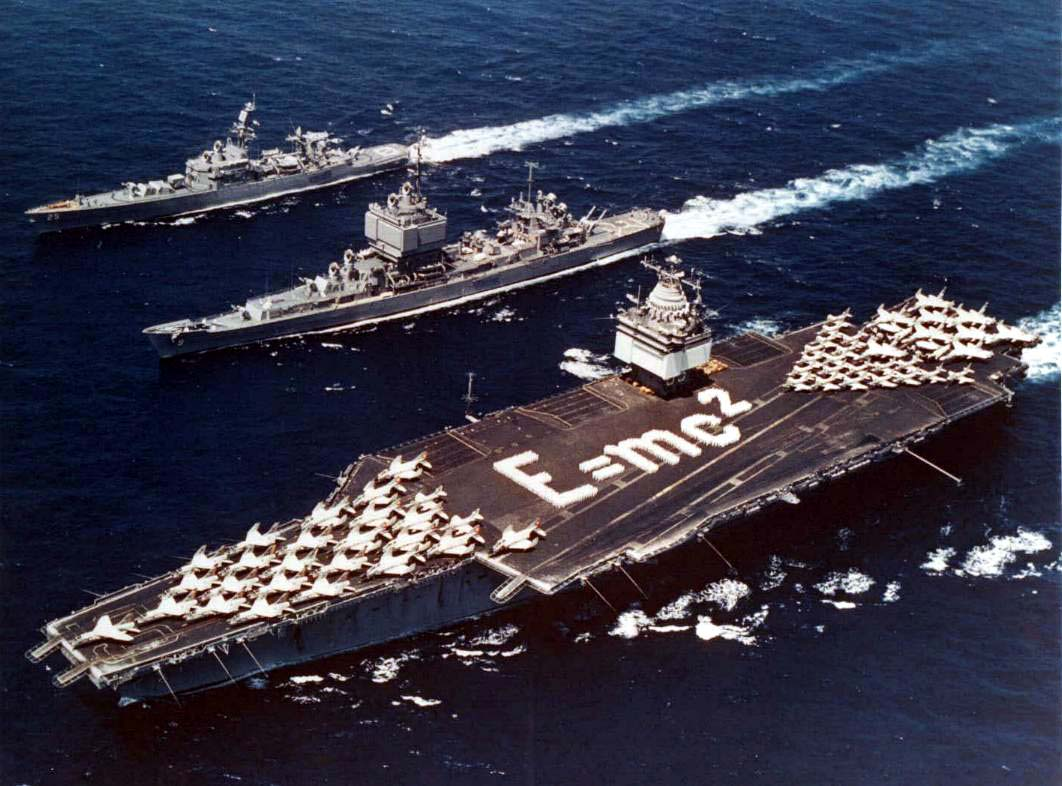
\includegraphics[width=0.7\textwidth]{enterprise}
	\caption{The crew of the USS Enterprise spell out $E = mc^2$ as she sets sail
around the world with similarly nuclear powered USS Long Beach and USS
Bainbridge on Operation Sea Orbit, 31 July, 1964 (There are also 3 submarines in
this picture.)}
\label{fig:enterprise}
\end{figure}

\section{Technology Description}
\subsection{Instrumentation and Control (I\&C) Systems}

The ability to control a nuclear reaction ultimately \textit{boils down} to managing the energy released from an unstable element that, once stimulated, emits both fast and slow neutrons. These neutrons go on to strike other fissile atoms, triggering further emissions in a self-sustaining chain reaction. This process takes place within fuel elements—long metal-clad rods arranged in a structure called a fuel subassembly, often resembling a metallic honeycomb. Multiple subassemblies are grouped into fuel assemblies, with careful placement to balance the resulting heat flux from neutron collisions. As neutrons scatter and interact, they excite more fuel atoms in a cascading effect reminiscent of a Fourth of July fireworks finale.

A simplified chemical representation of the process is the fission of uranium-235:

\begin{equation}
  ^{235}\text{U} + ^{1}\text{n} \rightarrow ^{92}\text{Kr} + ^{141}\text{Ba} +
	\text{\textbf{3}}^{1}\text{n} + \text{Energy}~(\approx 200~\text{MeV})
\end{equation}

\noindent where:
\begin{itemize}
  \item $^{235}\text{U}$ is a fissile uranium-235 nucleus,
  \item $^{1}\text{n}$ is an incoming thermal neutron,
  \item $^{92}\text{Kr}$ and $^{141}\text{Ba}$ are fission products,
  \item $3^{1}\text{n}$ represents the emission of three additional neutrons,
  \item The energy released is approximately 200~MeV, primarily as kinetic energy of the fission fragments and secondary neutrons.
\end{itemize}

These additional neutrons can go on to initiate further fission reactions, forming the basis of a self-sustaining chain reaction. The ability to keep this chain reaction in balance—neither accelerating nor dying out—is at the heart of nuclear reactor control.

The danger, however, lies in the potential for this excitation to grow out of control. The extent to which the system is primed for further reaction is measured as \textit{reactivity}, defined approximately as:

\begin{equation}
  \rho = \frac{k_{\text{eff}} - 1}{k_{\text{eff}}}
\end{equation}
where $\rho$ is the reactivity (dimensionless), $k_{\text{eff}}$ is the effective neutron multiplication factor and will increase in power unless corrective action is taken.

Advanced instrumentation and control (I\&C) systems are designed to maintain this reactivity within safe limits—keeping the metaphorical fireworks display safely choreographed in the sky rather than detonating all at once in a catastrophic burst at ground level.

To understand why these systems have evolved into such complex and nuanced architectures, it’s helpful to explore the different reactor design types. Over the decades, engineers have developed multiple ways to control reactivity and convert the energy from a “hot rock” into mechanical power—whether to propel submarines, generate electricity, or, in darker moments of history, to build devastating weapons.

\subsubsection*{Types of Plants}

Nuclear power plants can be classified by several characteristics, the most common being the type of coolant used to extract thermal energy from the reactor core. Table~\ref{tab:planttypes} categorizes four typical designs. Each has unique thermodynamic cycles and control architectures that dictate the required instrumentation, logic systems, and safety interlocks.

\begin{table}[H]
  \centering
  \caption{Types of Nuclear Power Plants \cite{ichandbook}}
  \label{tab:planttypes}
  \begin{tabular}{|c|c|c|}
    \hline
    \textbf{Reactor Type} & \textbf{Coolant Medium} & \textbf{Neutron Moderator} \\
    \hline
    Pressurized Water Reactor (PWR) & Light Water & Light Water \\
    Boiling Water Reactor (BWR) & Light Water & Light Water \\
    Heavy Water Reactor (CANDU) & Heavy Water (D$_2$O) & Heavy Water (D$_2$O) \\
    Advanced Gas-cooled Reactor (AGR) & CO$_2$ or Helium & Graphite \\
    \hline
  \end{tabular}
\end{table}

While this paper emphasizes PWR and BWR systems—depicted in Figures~\ref{fig:coreinstrumentation} and \ref{fig:bwrinstrumentation}—reactors can also be categorized by neutron energy spectrum (thermal, intermediate, fast), fuel configuration (homogeneous or heterogeneous), purpose (research, power, breeding, or plutonium production), and net fissile yield (breeder vs.\ converter) \cite{ichandbook}.

\subsubsection*{Reactor Monitoring Principles}

Instrumentation systems in nuclear power plants are designed to provide real-time, high-fidelity data on the most critical plant variables—particularly those affecting core reactivity, heat transfer, and plant integrity. These systems rely on a combination of neutron radiation sensors and thermal sensors, with sensor placement tailored to reactor type, as shown in Figures~\ref{fig:coreinstrumentation} and \ref{fig:bwrinstrumentation}.

\begin{figure}[H]
  \centering
  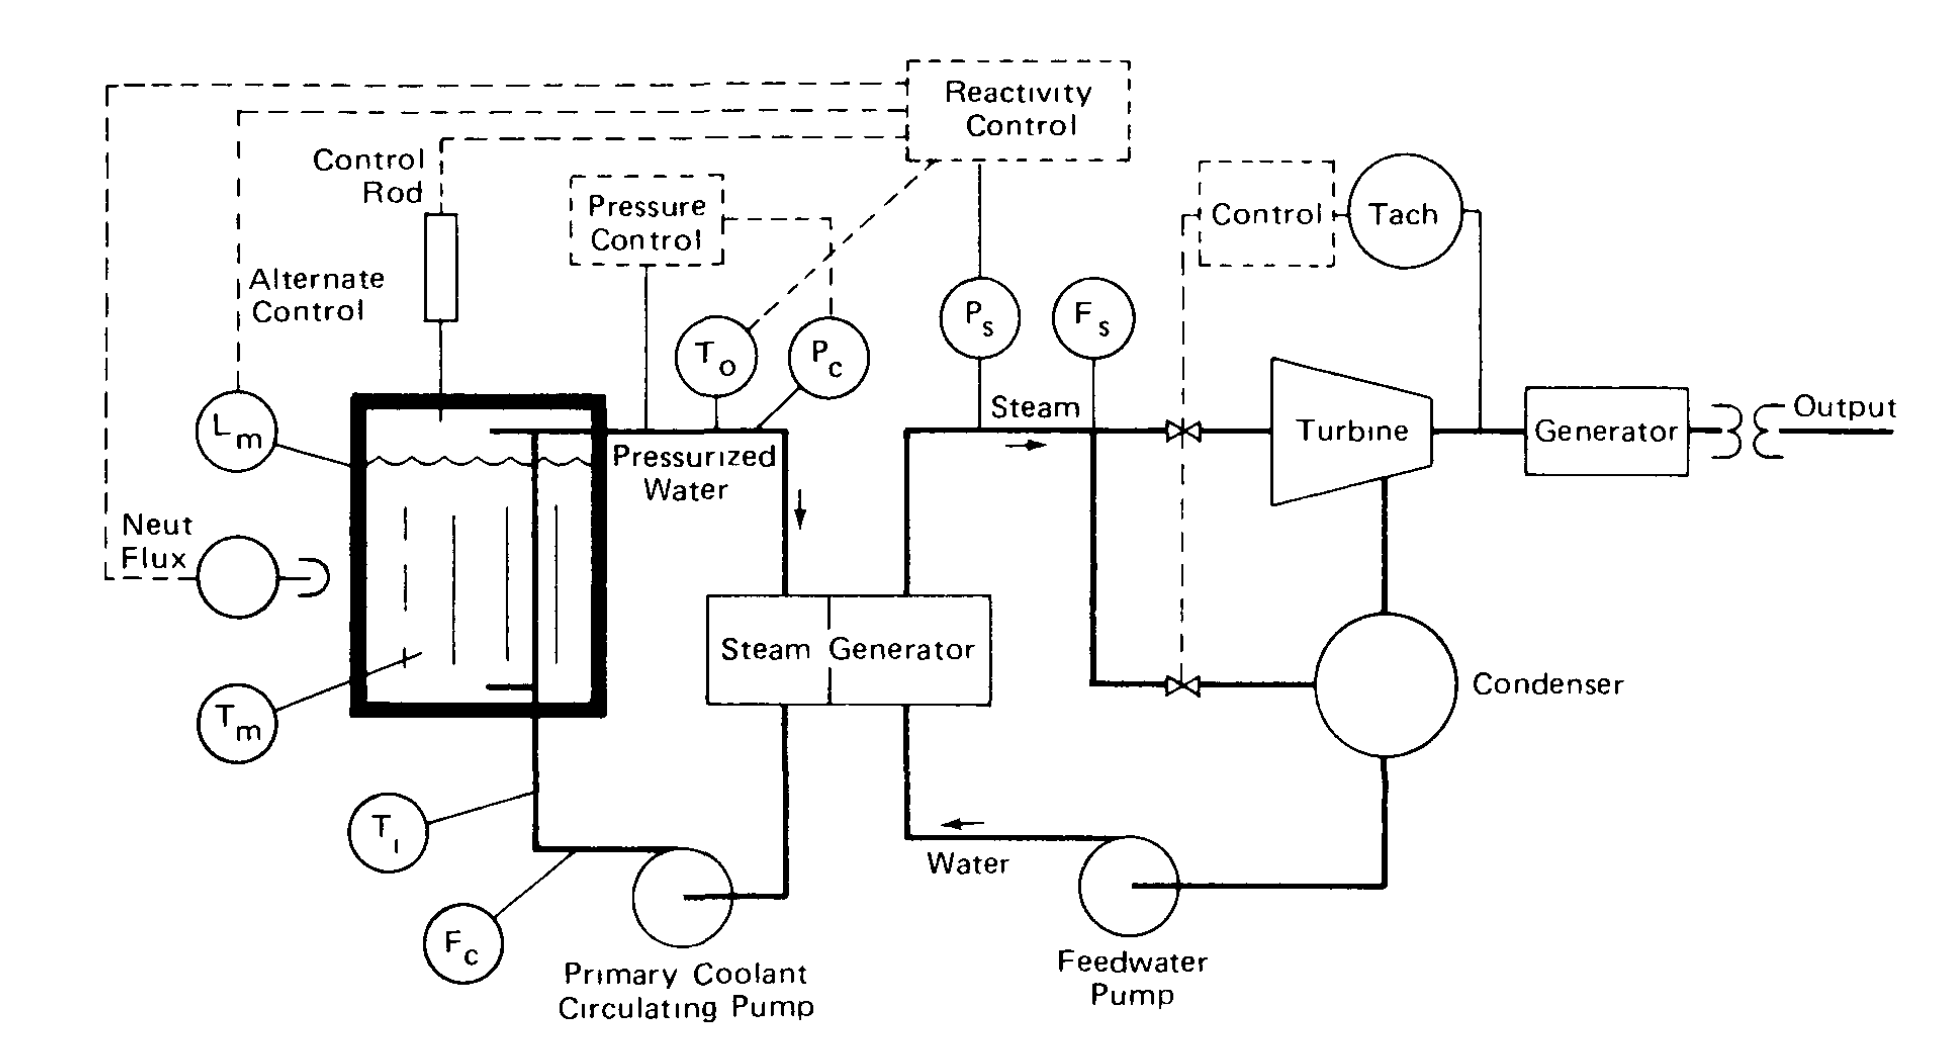
\includegraphics[width=0.75\textwidth]{instrumentation}
  \caption{Instrumentation layout for a typical PWR core \cite{nuctech}.}
  \label{fig:coreinstrumentation}
\end{figure}

\begin{figure}[H]
  \centering
  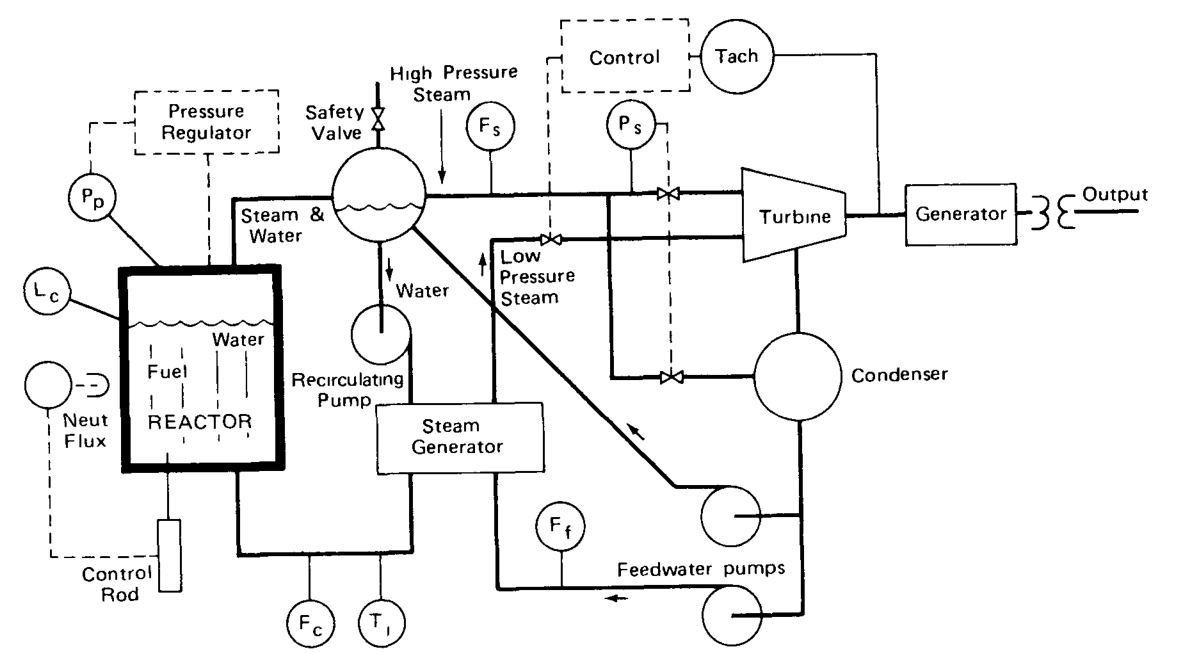
\includegraphics[width=0.75\textwidth]{bwr}
  \caption{Instrumentation layout for a typical BWR core \cite{nuctech}.}
  \label{fig:bwrinstrumentation}
\end{figure}

\subsubsection*{Thermal and Neutron Sensing.}
Sensors for nuclear plant monitoring fall broadly into two categories: thermal sensors and nuclear-radiation sensors \cite{ichandbook}. Thermocouples and resistance temperature detectors (RTDs) monitor coolant temperatures and structural heat loads, while neutron sensors directly measure fission activity. Because neutrons are uniquely tied to the fission process, neutron flux detectors are essential for monitoring power distribution, total fission rate, and the rate of change of reactor power.

\subsubsection*{Coolant and Moderator Instrumentation.}
Effective thermal management is essential to maintaining reactor integrity. The coolant serves as the medium for heat removal from the fuel, while the moderator governs neutron energy and thus reactivity. Continuous monitoring of coolant and moderator parameters ensures that the reactor operates within safe thermal limits and that reactivity remains controlled. Key measurements include \autocite{ichandbook}:
\begin{itemize}
  \item Coolant inlet and outlet temperatures (to track heat extraction).
  \item Flow rate into and out of the reactor ($F_c$), as well as through various coolant channels.
  \item Coolant pressure in both the core and outlet piping.
  \item Purity of coolant and its radioactivity, especially post-core.
  \item Moisture content (for gas-cooled systems), which may influence reactivity and heat transfer.
\end{itemize}
These measurements require temperature sensors, flowmeters, pressure transducers, gamma sensors, and humidity detectors. In light water reactors, precise detection of subcooled margin, void fraction, and departure from nucleate boiling (DNB) is paramount to prevent fuel damage and ensure efficient heat transfer.

\subsubsection*{Control and Structural Monitoring.}
To maintain criticality and prevent excursions, the physical state of reactor components must be known at all times. This includes not only the position of reactivity control elements like control rods, but also the condition of structural moderators and pressure boundaries. Accurate readings in this domain allow for dynamic reactivity management, prompt detection of abnormal trends, and safe system operation:
\begin{itemize}
  \item Position of control rods ($L^*$), crucial for reactivity control.
  \item Moderator and reactor water levels ($L_m$, $L_r$).
  \item Moderator temperature ($T_m$), especially in systems like CANDU reactors.
  \item Primary system pressure ($P_p$) and coolant outlet pressure ($P_o$).
\end{itemize}
These parameters are sensed via linear variable differential transformers (LVDTs), water-level probes, and high-accuracy pressure transducers. Their outputs are often fed into automated feedback loops and supervisory control systems.

\subsubsection*{Steam and Turbine System Sensing.}
Instrumentation extends beyond the core into the balance-of-plant systems where thermal energy is converted into mechanical and electrical power. Monitoring the secondary loop ensures safe and efficient energy extraction, minimizes mechanical wear, and protects the grid interface. Key measurements include:
\begin{itemize}
  \item Steam flow rate ($F_s$), steam quality, and pressure ($P_g$).
  \item Feedwater flow ($F_f$) and drum level (in BWRs).
  \item Turbine rotational speed, generator output power, and pump motor performance.
\end{itemize}
These measurements are collected using tachometers, electrical metering, differential pressure sensors, and dynamic vibration monitors. They are vital for maintaining power stability, avoiding turbine overspeed or cavitation, and ensuring that thermal energy is extracted as efficiently and safely as possible.

\subsection{Automatic Protection}
The increasing integration of digital logic enables centralized monitoring of these diverse parameters using high-speed buses and distributed control systems (DCS). Such systems can perform real-time diagnostics, apply fail-safe logic, and enhance overall plant safety and responsiveness.

These layered instrumentation systems—distributed across reactor, coolant, and steam systems—are designed to uphold the three core principles of nuclear safety: maintain reactivity control, ensure heat removal, and prevent release of radioactive materials. The careful selection and redundancy of sensors make them foundational to modern nuclear plant reliability.

\subsubsection*{Computerized Protection Systems}
\label{sec:protection}

The progression toward digital protection systems has paralleled improvements in reactor safety and reliability. Engineered safety features (ESFs) are now fully integrated with digital I\&C, simplifying operational logic through pre-programmed safety interlocks. These include automated trip logic and permissives designed to act faster than human operators during transient conditions \cite{moderninstruments}.

\begin{itemize}
  \item \textbf{SCRAM}: Rapid insertion of control rods into the reactor core to immediately terminate the chain reaction.
  \item \textbf{Pressure Relief Valves}: Automatic venting of steam or water to prevent overpressurization in the primary loop.
  \item \textbf{High/Low Pressure Trips}: Activate a SCRAM if loop pressure deviates beyond specified design tolerances.
  \item \textbf{Coolant Flow Trips}: Triggered by low primary loop flow, protecting against core overheating and fuel damage.
  \item \textbf{Temperature Differential Trips}: Monitor the hot leg and cold leg of the primary loop; trip the reactor if temperature gradients exceed safe limits.
  \item \textbf{Pressurizer Heater Control}: Automatic cycling of heaters to maintain loop pressure during load changes.
\end{itemize}

Figure~\ref{fig:flowlogic} shows a representative logic diagram for a U.S.-based plant, illustrating how these subsystems are interlinked for layered protection.

\begin{figure}[H]
  \centering
  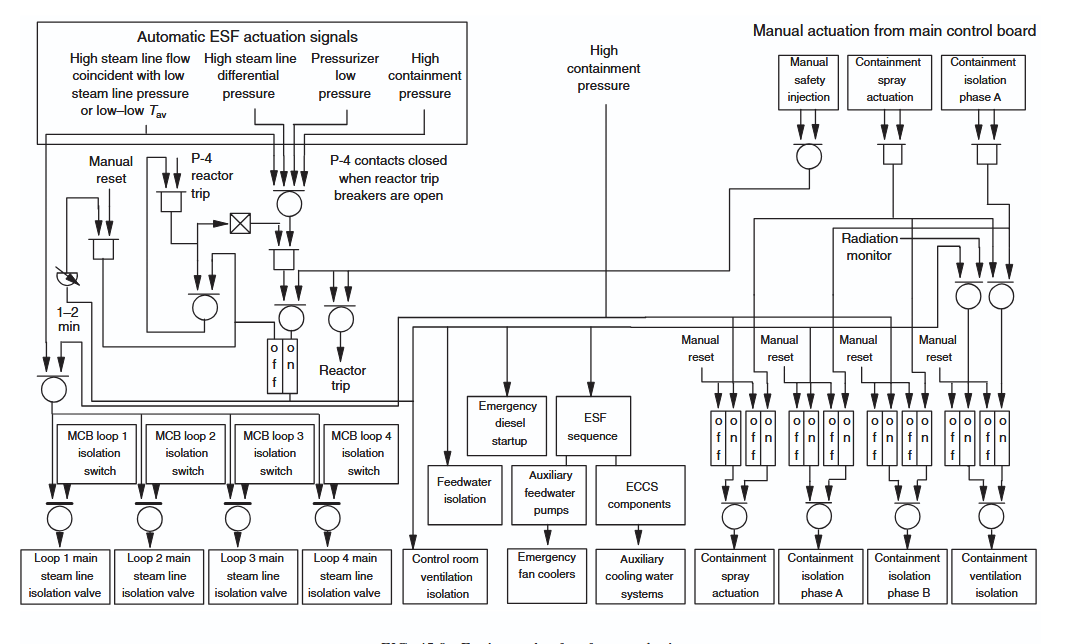
\includegraphics[width=0.95\textwidth]{safetylogic.png}
  \caption{Representative reactor safety logic for a U.S. plant \cite{moderninstruments}.}
  \label{fig:flowlogic}
\end{figure}

Critically, such systems are not intended for routine plant operation. Instead, their design assumes operator control remains primary and that automated systems intervene only during design-basis accidents or unanticipated transients. For example, while a pressurizer may tolerate pressures from \SI{1500}{psig} to \SI{2500}{psig}, licensed operators will typically maintain nominal pressure near \SI{2250}{psig}\footnote{These numbers are shown purely for example and not based on existing plant design.} to ensure that automatic systems are not actuated unless multiple control layers fail.

Ultimately, these protection systems provide defense-in-depth and are structured around the core nuclear safety principles: control of reactivity, heat removal, and containment of radioactive materials. The move to digital logic enhances responsiveness but demands rigorous validation, fail-safe architectures, and operator situational awareness to maintain overall plant safety.

\section{Broader Impacts}
To understand the foundation of modern nuclear safety, it is essential to examine key historical nuclear accidents. These events, extensively studied both in naval reactor training and across the commercial nuclear sector, highlight the serious risks inherent to nuclear technology when safety systems fail. The lessons drawn from these incidents have directly influenced the development of today’s robust safety frameworks.

Following this overview, the section explores the broader environmental, economic, and societal consequences of these accidents. It discusses how public perception and regulatory response have shaped the trajectory of nuclear power over recent decades, contributing to its slowed adoption despite technological advancements.

\subsection{Historical Lessons in Reactor Safety}
\label{sec:accidents}

\subsubsection*{SL-1: The First Fatal U.S. Reactor Accident}

On January 3, 1961, the Army’s Stationary Low-Power Reactor Number One (SL-1) experienced the first fatal nuclear accident in U.S. history. During routine maintenance, the manual withdrawal of a control rod made the small test reactor prompt critical, leading to a steam explosion that destroyed the core and killed all three personnel on duty \autocite{sl1report}. Figure~\ref{fig:sl1diagram} shows the post-incident state of the reactor vessel.

\begin{figure}[H]
    \centering
    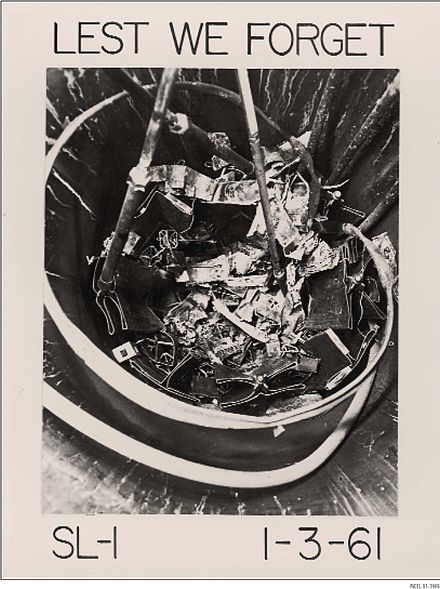
\includegraphics[width=0.35\textwidth]{sl1diagram.jpg}
    \caption{The damaged SL-1 reactor core following the prompt critical excursion \autocite{sl1report}.}
    \label{fig:sl1diagram}
\end{figure}

SL-1 used top-mounted control rods for reactivity control, which were manually withdrawn during maintenance procedures. Operators had previously documented that rods frequently stuck due to thermal expansion of the drive mechanisms. It became common to exert above-normal force during removal. On the night of the accident, the center control rod—the most reactivity-dominant—was pulled upward over 50 centimeters in a single motion, far beyond the safe insertion limit. The resulting reactivity spike caused a runaway chain reaction and a destructive power surge in under 4 milliseconds \autocite{sl1report}.

Despite repeated reports of sticking rods, the system lacked mechanical or
procedural interlocks to prevent rapid withdrawal. A single operator retained
full manual control, with no redundancy or supervisory lockouts. The SL-1 event
shows the critical role of human factors engineering, particularly in minimizing
design interfaces (IE maintenance procedures) that allow unsafe manual operations.

\subsubsection*{Three Mile Island: Interface Confusion and Human Factors}
The Three Mile Island Unit 2 (TMI-2) accident occurred on March 28, 1979, near Harrisburg, Pennsylvania, and remains the most serious commercial nuclear accident in the United States. It was precipitated by the failure of a pressure-operated relief valve (PORV) that became stuck open during a minor malfunction. The valve allowed coolant to escape from the pressurizer, but due to inadequate instrumentation, operators believed it had closed properly \autocite{tmiwalker}.

The event began with a relatively minor mechanical issue: a malfunction in the
secondary cooling system caused the reactor to automatically shut down. In
response, the PORV opened to relieve pressure but failed to reseat. As coolant
escaped from the system, the core began to overheat. However, operators—faced
with a cascade of alarms and ambiguous signals—misinterpreted the problem.
Believing the system to be overpressurized, they manually shut off the emergency
core cooling system (ECCS), thereby worsening the core heat-up. This operator
action, based on incomplete and confusing data, allowed the core to partially
melt. The confusing control room can be seen in Figure~\ref{fig:tmicontrolroom}.

\begin{figure}[H]
  \centering
  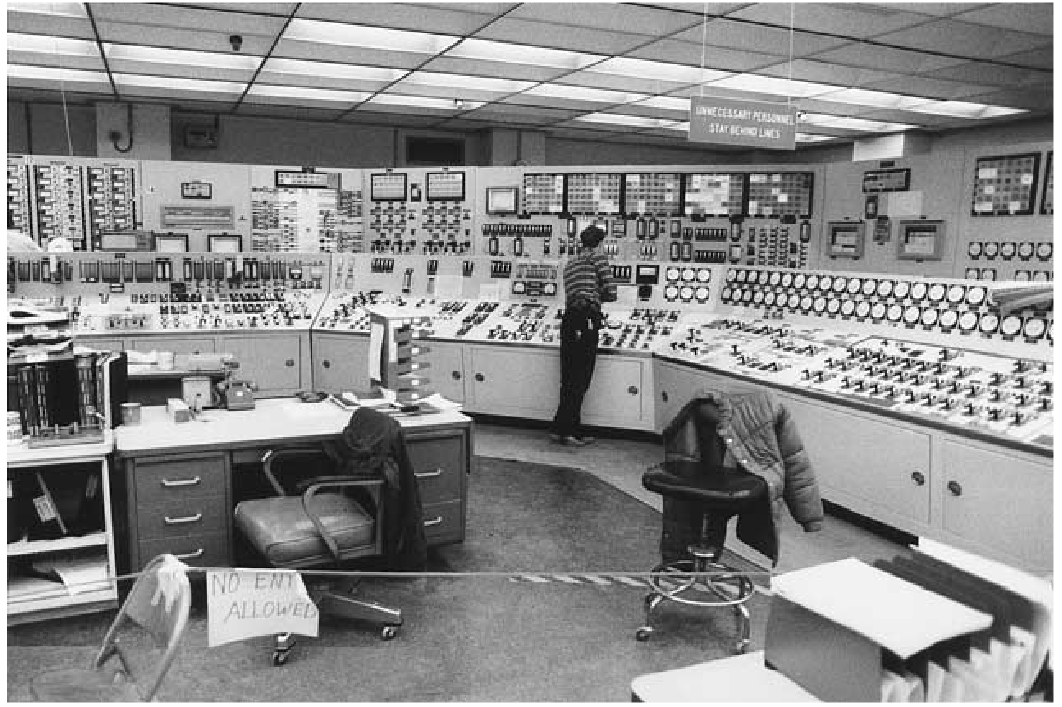
\includegraphics[width=0.75\textwidth]{tmicontrolroom.png}
  \caption{The control room of TMI-2 on April 3, 1979, following the accident \autocite{tmiwalker}.}
  \label{fig:tmicontrolroom}
\end{figure}

Prior to this event, the relationship between human performance and system design was underappreciated in reactor control engineering. It was often assumed that proper training and “common sense” would be sufficient for managing system faults. However, the TMI-2 accident highlighted that even well-trained operators can make catastrophic errors when systems are not designed to support human cognition under stress.

As a result of this accident, the field of human factors engineering gained
legitimacy within the nuclear industry. Organizational and industrial
psychology—especially the study of ergonomics and operator-centered
design—emerged as crucial disciplines in instrumentation and control system
development \autocite{meshkati1991human}. Operators needed interfaces not merely
for function, but for situational awareness and decision-making under pressure.
This marked a turning point in control room design philosophies, ushering in
era-defining updates to alarm management, display hierarchy, and interface logic
\autocite{moderninstruments}. This will be explored thoroughly in
Section~\ref{sec:humanfactors}

\subsubsection*{Chernobyl and Reactor Design Faults}

The catastrophic accident at Chernobyl's Reactor No.~4 occurred on April 26, 1986, during a late-night safety test. The test intended to verify whether the rotational inertia of the turbine could temporarily power the emergency coolant pumps in the event of a grid power failure \autocite{wna2023chernobyl}. The RBMK-1000 reactor involved was a Soviet-designed graphite-moderated, water-cooled system—flawed by both design and execution \autocite{iaea1992chernobyl, nrc_chernobyl}.

Ordinarily, a SCRAM should halt a reaction. However, the RBMK rods featured graphite tips that displaced neutron-absorbing water before inserting the boron carbide absorber sections. This caused a momentary \textit{increase} in reactivity in the lower portion of the core, leading to a rapid, uncontrollable rise in power. The reactor reached a prompt critical state within seconds \autocite{iaea1992chernobyl}.

The core overheated instantly, rupturing fuel channels and vaporizing coolant. A violent steam explosion lifted the reactor’s 2,000-ton upper biological shield. A second explosion—possibly from hydrogen or steam—further breached the structure and exposed the graphite moderator, which caught fire. Figure~\ref{fig:chernobylafter} shows the aftermath of the explosion mere hours after the explosion. The fire lofted radioactive particles into the upper atmosphere, affecting much of Europe \autocite{nrc_chernobyl}.

\begin{figure}[H]
  \centering
  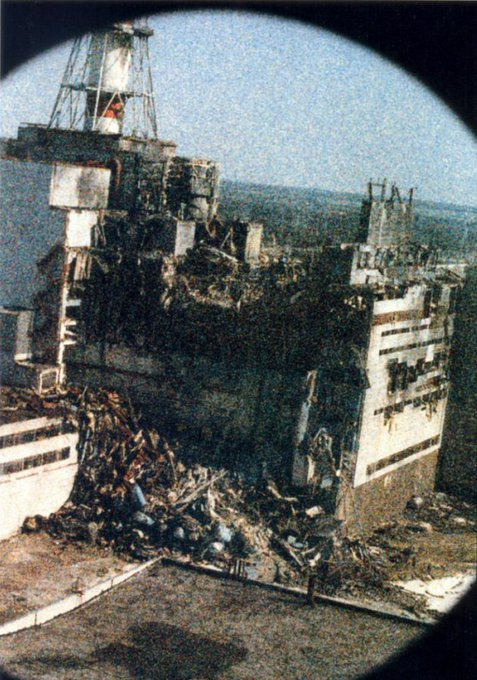
\includegraphics[width=0.45\textwidth]{chernobylafter.jpg}
  \caption{Chernobyl Reactor No.~4 on April 27, 1986, 14 hours after the explosion \autocite{medvedev1991truth}.}
  \label{fig:chernobylafter}
\end{figure}

The aftermath of Chernobyl catalyzed global reevaluation of nuclear safety, reactor design, and operator training. The international community pushed for increased transparency, safety audits, and enhanced containment strategies. The photograph in Figure~\ref{fig:elephantsfoot} famously shows the “Elephant’s Foot,” a deadly corium formation. The strange visual static in the image is not lightning, but film degradation from intense radiation—testament to the unprecedented radioactive environment at the site.

\begin{figure}[H]
  \centering
  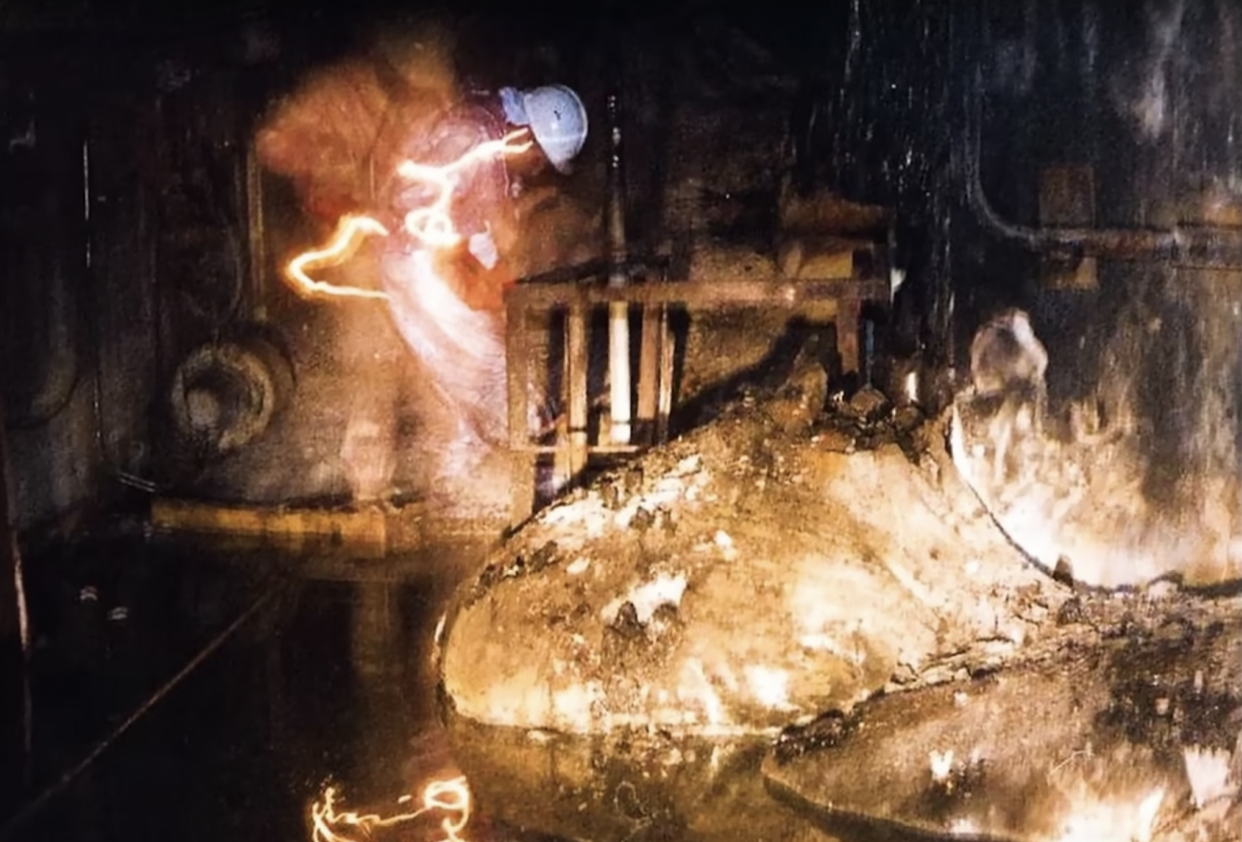
\includegraphics[width=0.5\textwidth]{elephantsfoot.png}
  \caption{The ``Elephant’s Foot'': a mass of corium under Reactor No.~4, composed of melted fuel, sand, and reactor structural materials \autocite{medvedev1991truth}.}
  \label{fig:elephantsfoot}
\end{figure}

The disaster marked a permanent shift in public perception of nuclear energy,
influencing decades of policy and triggering a global slowdown in nuclear
development. This politically changed the entire world's perception of the
potential for ``Safe Nuclear Power" and will be discussed in
Section~\ref{sec:infrastructure}.


\subsubsection*{Fukushima-Daiichi: Environmental Consequences}

On March 11, 2011, a magnitude 9.0 undersea megathrust earthquake struck off the northeastern coast of Honshu, Japan, triggering a tsunami with wave heights exceeding 14 meters. The Fukushima-Daiichi Nuclear Power Station, operated by TEPCO, was critically affected. Although the three operating reactors—Units 1, 2, and 3—successfully SCRAMed, the tsunami flooded the site and disabled both the offsite grid connections and emergency diesel generators \autocite{iaea_fukushima_report}. This unprecedented loss of power across all units is illustrated in Figure~\ref{fig:containments}, which shows the reactor buildings after successive hydrogen explosions.

\begin{figure}[H]
  \centering
  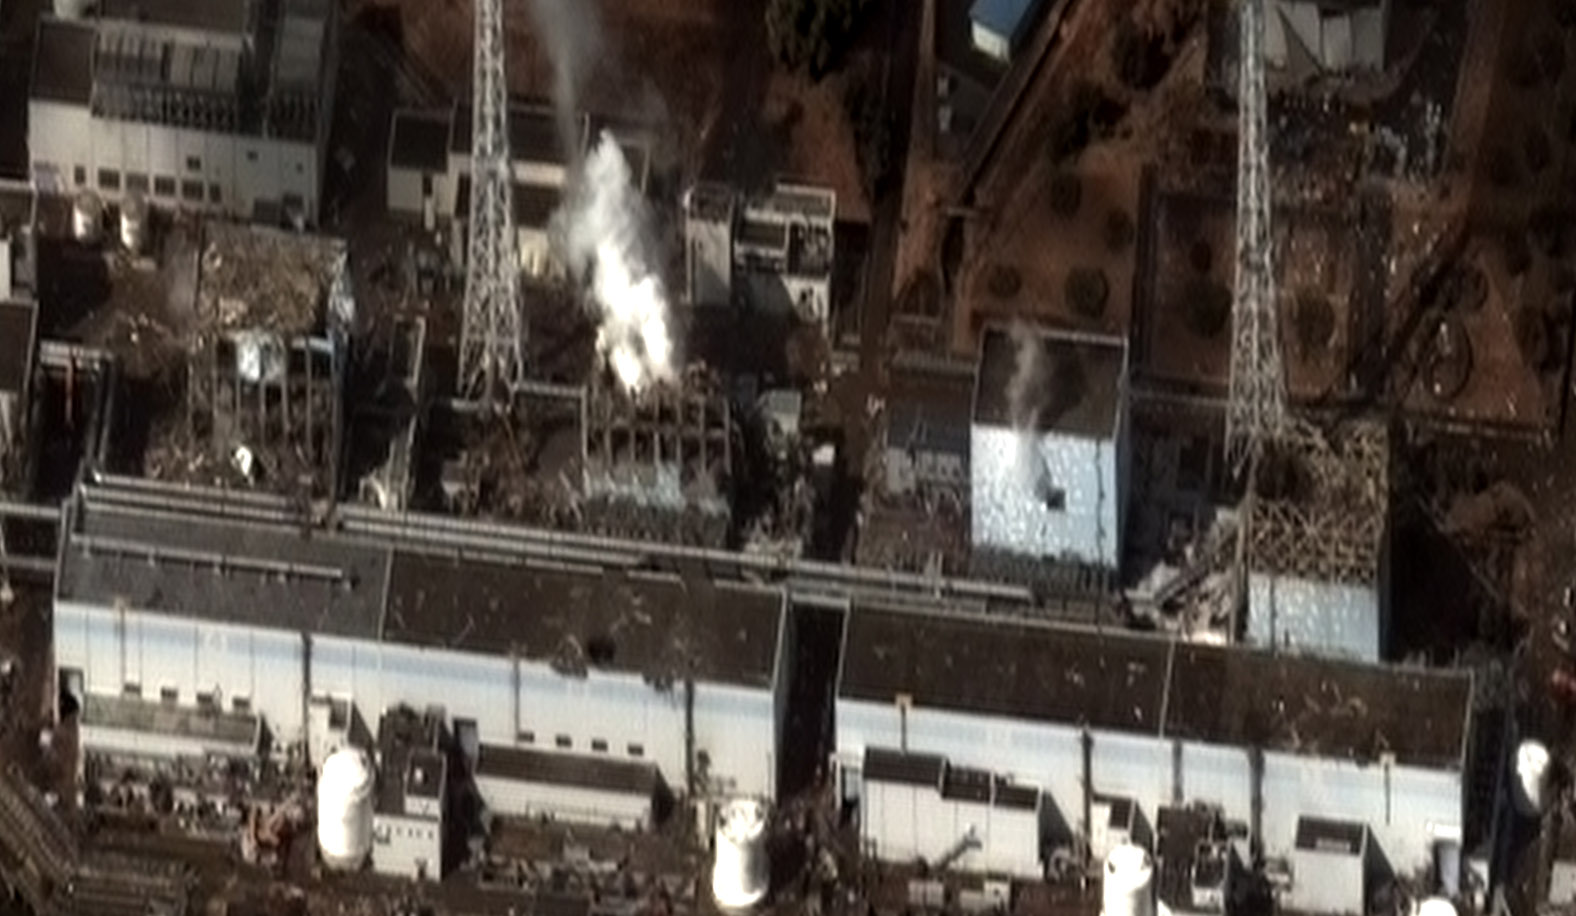
\includegraphics[width=0.5\textwidth]{fukushimaafter.jpg}
  \caption{Fukushima-Daiichi Nuclear Power Station: The four damaged reactor containments (from left: Units 4, 3, 2, and 1) on 16 March, 2011 \autocite{worldnuclear_fukushima_review}.}
  \label{fig:containments}
\end{figure}

Following shutdown, nuclear reactors continue to emit decay heat, which can exceed several percent of nominal thermal power in the hours after fission halts. This residual heat must be actively removed to avoid core damage. At Fukushima, all cooling systems failed due to the flooding of diesel generators and electrical switchgear—many of which were located in basements vulnerable to tsunami inundation \autocite{nrc_fukushima}. This left the plant in a condition known in the nuclear industry as \textit{dead electric}, where no AC or DC power is available to operate pumps, valves, or even basic monitoring systems.

Operators at Fukushima recognized the danger but were rendered effectively blind by the loss of power. Unlike U.S. Navy reactor systems—where portable test equipment such as Fluke digital multimeters can be attached to terminals for passive thermocouple readings—the Fukushima design lacked redundant manual monitoring options. In a desperate act of ingenuity, personnel retrieved car batteries from nearby vehicles and wired them in series to restore minimal voltage to power essential instrumentation. Unfortunately, by the time this improvised power source was implemented, core damage in Units 1, 2, and 3 was already underway, with partial or full meltdown confirmed in post-event analyses \autocite{worldnuclear_fukushima_review}.

\subsection{Human Factors: The Ethical Dimension of Automation}
\label{sec:humanfactors}

The role of trained human operators in the safe and reliable generation of nuclear power cannot be overstated. Despite vast improvements in automation, instrumentation, and control systems, the nuclear accidents at SL-1, Three Mile Island, Chernobyl, and Fukushima-Daiichi demonstrate that the human element remains indispensable. These incidents demonstrate the importance of sound judgment, situational awareness, and expert intervention when systems fail or behave unpredictably \autocite{moderninstruments}.

\textit{Human factors engineering} (HFE) is the systematic application of knowledge about human capabilities, limitations, behaviors, and interactions to the design of systems, equipment, and tasks. In the nuclear industry, HFE plays a vital role in ensuring that complex control systems support rather than hinder operator performance—especially in high-pressure situations.

Key elements of human factors integration include the reliable \textit{presentation of information}, \textit{uniform control design}, well-thought-out \textit{panel and display layouts}, and procedural integration via \textit{full-scope simulators} that replicate real plant conditions \autocite{iec60964, iec964}.

\subsubsection*{Operator Experience}
While engineering design establishes operational parameters, it is the operator who understands the plant in real time. Experienced operators know how the system responds to subtle inputs—such as a one-second control rod shim or a \SI{10}{psig} fluctuation in secondary steam pressure. Similarly, machinery room technicians can predict how valve sequencing will affect temperature, flow, or turbine response.

In early prototype plants, small reactor cores were operated at constant loads
by teams of scientists and engineers pushing the limits of atomic knowledge
\autocite{moderninstruments}. As commercial nuclear power scaled up, these
systems became vastly more complex, and measurement accuracy and control
precision grew increasingly important. Figure~\ref{fig:maneuvering} shows
experienced operators aboard an S5W-era submarine in a shutdown configuration.
\begin{figure}[H]
	\centering
	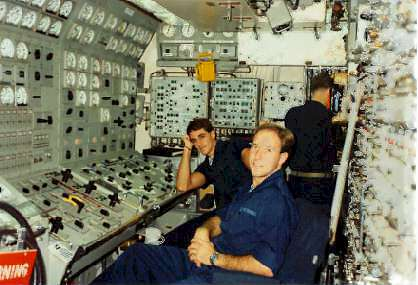
\includegraphics{maneuvering-watch.jpg}
	\caption{The small cramped room in a nuclear submarine named maneuvering, in
	the front is the Shutdown Reactor Operator, and to his right is the Electrical
Operator.}
	\label{fig:maneuvering}
\end{figure}

Modern operators are trained not only on procedural execution but also on pattern recognition, anomaly detection, and adaptive response. Their insights cannot be easily modeled or coded into automation algorithms, especially under degraded conditions or unforeseen emergencies.

\subsubsection*{The Danger in Automation}
While automation has dramatically improved reactor safety, it must be implemented with caution. In certain crisis scenarios, reliance on preprogrammed logic or incomplete models may lead to incorrect or delayed actions. Ethical considerations demand that humans remain at the center of safety-critical decisions, particularly when outcomes involve lives or large-scale environmental consequences.

One well-documented challenge in cognitive psychology is the \textit{tunnel effect}, in which humans persist with an initial, incorrect interpretation of a situation, especially under stress \autocite{moderninstruments}. This phenomenon is exacerbated when control system layouts are unintuitive or overwhelming. Retrofitting advanced instrumentation without corresponding operator retraining can invalidate experience and increase error likelihood.

Moreover, automated models are developed under assumptions that may no longer apply in aging plants. Changes to fuel characteristics, core configurations, or coolant flow paths can render original logic sequences obsolete. This can lead to spurious trips, false alarms, or missed safety signals—potentially costing a commercial plant lost megawatt-hours, or a naval reactor lost propulsion.

For these reasons, complete automation is neither practical nor desirable in contemporary nuclear power plants. A hybrid architecture—where human operators are empowered by automation, not replaced by it—is currently the safest and most reliable solution.

\begin{figure}[H]
  \centering
  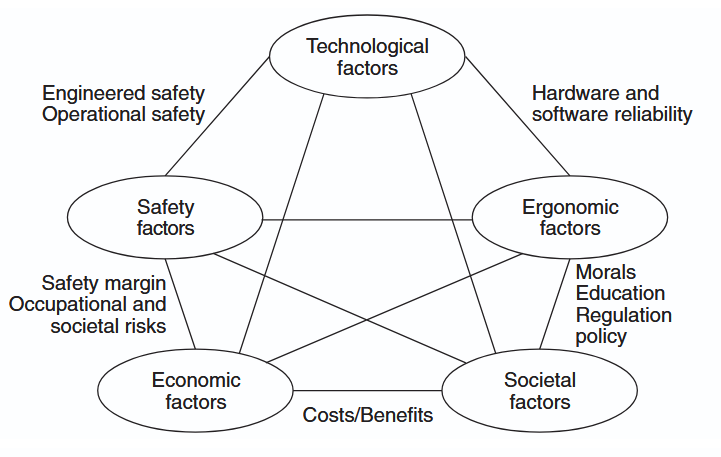
\includegraphics[width=0.5\textwidth]{automationfactors}
  \caption{Automation and human factors in nuclear power generation \autocite{moderninstruments}.}
  \label{fig:automationfactors}
\end{figure}

The optimal nuclear power plant integrates advanced control systems with a highly trained crew. These operators undergo continuous simulation training for casualty scenarios and are equipped with real-time diagnostic tools. Such a system ensures robust safety, resilience to abnormal events, and operational excellence.

\begin{figure}[H]
  \centering
  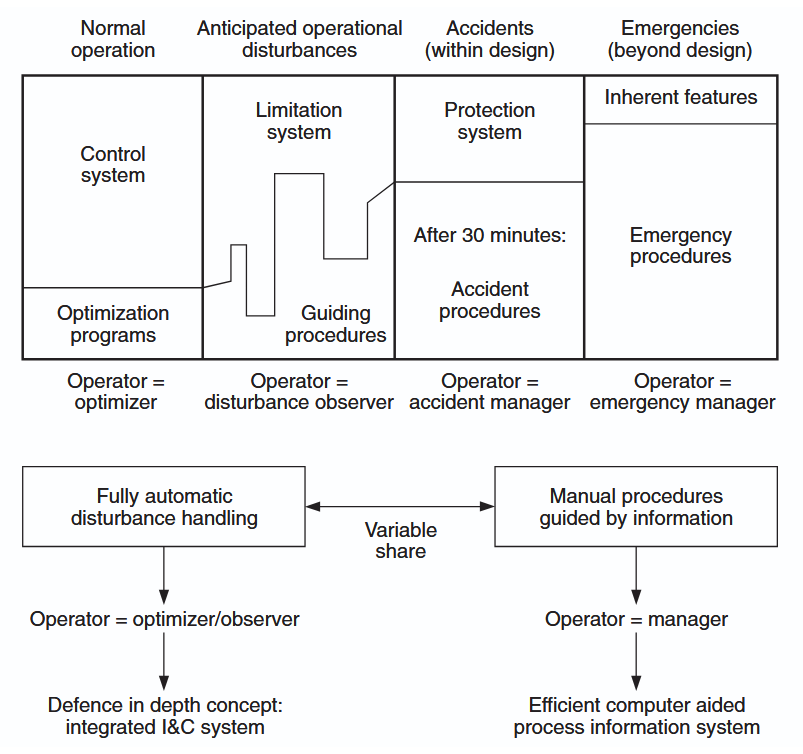
\includegraphics[width=0.5\textwidth]{optimalautomation.png}
  \caption{The optimal balance between automation and human factors in nuclear power generation \autocite{moderninstruments}.}
  \label{fig:optimalautomation}
\end{figure}

\subsection{Economic Realities and Infrastructure Decline}
\label{sec:infrastructure}

Due to the high-profile mishaps discussed in Section~\ref{sec:accidents}, the nuclear industry has suffered a significant loss of public trust. This erosion of confidence has contributed to financial uncertainty, stalled development, and a decline in domestic infrastructure to support new reactor construction. The resulting industrial contraction has drawn comparisons to the decline of the coal rail economy—once supported by a network of coal suppliers and rail hubs across the United States. As investment and skilled labor shift toward renewable energy, nuclear power is increasingly seen as an economically fragile legacy technology.

\subsection{Waste Management and Decommissioning Costs}
\label{sec:wastemanagement}

A commercial nuclear reactor undergoes refueling approximately every 18 to 24 months, with each cycle costing between \$50 million and \$100 million \autocite{wnisr2022}. These costs include fuel handling, transport logistics, containment, and licensing. Spent fuel is highly radioactive and must be isolated from the environment for thousands of years, necessitating complex storage and oversight systems.

The U.S. currently stores most of its spent fuel onsite in dry cask storage, as it lacks a permanent geologic repository. The proposed Yucca Mountain site in Nevada was halted due to political opposition, leaving a critical infrastructure gap \autocite{doe2020}. Meanwhile, the Department of Energy (DOE) estimates that total long-term waste management liabilities—including storage, monitoring, and decommissioning—could exceed \$500 billion over the next century \autocite{doe2020}. Several private firms that formerly handled nuclear logistics and fuel services have transitioned into renewable technologies or left the sector entirely, further weakening the industry’s support structure.

\subsection{Construction and Design of Future Plants: The Societal Impact}
The capability to construct new nuclear facilities has also diminished. The completion of Vogtle Unit~4 in Georgia—one of the first new U.S. reactors in decades—offered a glimmer of progress, but also exposed the harsh economic and logistical realities of modern nuclear construction. The project faced a decade of delays and billions in cost overruns, driven by labor shortages, supply chain gaps, and regulatory hurdles \autocite{aafnuclearcosts}.

Domestic capacity to manufacture nuclear-grade components, such as reactor pressure vessels or reactor coolant pumps, has eroded. Only a few specialized forges worldwide are still capable of producing these massive components to the necessary ASME and NRC specifications. Simultaneously, industrial firms that once supported nuclear projects have shifted their operations toward building wind turbine towers, solar inverters, and battery storage systems. The opportunity cost of investing in nuclear has grown as renewables offer faster return on investment and benefit from robust public and private incentives.

This migration is not merely market-driven; it is reinforced by regulatory environments. Post-Fukushima mandates have led to stricter safety requirements and more frequent inspections, raising compliance and licensing costs. Some U.S. plants face annual regulatory costs in excess of \$20 million \autocite{aafnuclearcosts}. These growing financial burdens make nuclear projects less attractive in both the public and private sectors.

Despite economic challenges, nuclear energy offers unique value as a source of stable baseload power. This makes it an ideal complement to intermittent renewable sources like wind and solar. However, current policy frameworks often prioritize short-term carbon reduction via rapidly deployable renewables, sidelining nuclear investments that require long lead times and upfront capital.

A salient example is the rise of offshore wind infrastructure in coastal cities such as New London, Connecticut. These projects attract federal and state subsidies, media attention, and educational investments, while nuclear plants are increasingly perceived as costly, inflexible, or outdated \autocite{abdussami2025future}.

Public perception remains a formidable barrier. While nuclear power remains one of the lowest-carbon energy sources per unit of energy generated, its association with catastrophic events has left a lasting impact on societal attitudes. Without substantial policy reform and education efforts, nuclear energy will remain economically disadvantaged despite its technical merits.

\section{Conclusion: A Cautious Return to the Atom}

Nuclear power stands at a complex crossroads—one defined by profound ethical obligations, hard-earned technological lessons, and a rapidly shifting energy landscape. The historical record, shaped by the tragic events at SL-1, Three Mile Island, Chernobyl, and Fukushima-Daiichi, offers clear testimony to the irreplaceable role of human judgment in reactor safety. These accidents remind us that automation, while powerful, must be designed with the understanding that it supports rather than supplants trained human operators.

Human factors engineering has evolved into a critical field, embedding psychological, ergonomic, and procedural insights directly into plant design. Simulators, intuitive control room layouts, and refined information presentation now stand as defenses against the tunnel vision and decision fatigue that so often accompany crises. The ethical responsibility to keep a human in the loop—especially in decisions with irreversible consequences—cannot be ignored, even as algorithms grow more capable and systems more autonomous.

Yet, the technical and economic challenges facing nuclear power are sobering. The decline of manufacturing capacity, the shuttering of legacy vendors, and the migration of talent and capital toward renewables have left the nuclear sector precariously under-resourced. Without consistent policy support and industrial reinvestment, the risk of losing irreplaceable expertise and infrastructure grows with each passing year. The lack of a permanent waste repository and the mounting costs of decommissioning further complicate the long-term viability of the industry.

Still, all is not lost. Projects like Vogtle Units~3 and~4 in Georgia—despite cost overruns and delays—signal a possible turning point. They represent not only a technological achievement but also a renewal of confidence in the idea that nuclear energy can still play a vital role in our decarbonized future. The emergence of small modular reactors (SMRs), the refinement of passive safety designs, and renewed global interest in energy resilience have reinvigorated the conversation.

To move forward, we must blend the hard-won wisdom of past experience with the innovative tools of modern engineering. Nuclear power will never be perfect—but neither is any energy source. What makes it unique is the immense power it offers, not just in megawatts, but in the philosophical sense: a force that must be handled with reverence, precision, and foresight. The atom, split with care and humility, may yet illuminate a sustainable and responsible path forward.\footnote{An LLM was used strictly for formatting IAW IEEE Editorial Style Manual
	for Authors. All thoughts, prose, and conclusions are
my own.}
\newpage
\addcontentsline{toc}{section}{References}
\begingroup
\sloppy
\printbibliography
\endgroup

\end{document}
% vim: set ft=tex tw=80 ts=2 sts=2 sw=2 noet spell:
